\subsection{Geometry editor}
\label{sec:sf-geometry}
\writer{Mikko}

The Geometry Editor is a component that will allow the user to create and edit geometry models. Such models consist of geometry objects, namely \textit{lines} and \textit{points} and are defined as a two dimensional representation of the Petri net objects to be simulated. The connection between the geometry and the Petri net objects will be done via the \textit{geometry labels}.

\subsubsection{Functional Requirements}

\begin{enumerate}
	\item The Geometry Editor \textbf{shall} allow the user to create, edit and delete points.
	\item The Geometry Editor \textbf{shall} allow the user to define points as Input Point, Connector or Bend Point.
	\item The Geometry Editor \textbf{shall} allow the user to create, edit and delete lines.
	\item The Geometry Editor \textbf{shall} allow the user to load and save geometry files.
	\item The Geometry Editor \textbf{shall} allow the user to define labels for geometry objects.
	\item The Geometry Editor \textbf{shall} allow the user to define appearance labels for Lines and Input Points.
	\item The Geometry Editor \textbf{should} allow the user to create curved lines.
	\item The Geometry Editor \textbf{should} allow the user to create, edit and delete bend points for the lines.
	\item The Geometry Editor \textbf{should} allow the user to use undo and redo.
	\item The Geometry Editor \textbf{should} allow user to use copy, paste and cut geometry objects.
	\item The Geometry Editor \textbf{should} have drag and drop interface.
	\item It \textbf{would be nice} if the Geometry Editor allowed the user to create different kinds of parametric curved lines, such as Catmull-rom spline and Bézier-curves.
	\item It \textbf{would be nice} if the Geometry Editor allowed the user to zoom and pan the geometry canvas.
	\item It \textbf{would be nice} if the Geometry Editor allowed the user select multiple geometry objects simultaneously.
	\item It \textbf{would be nice} if the Geometry Editor allowed the user to load multiple geometries on same canvas.
	\item It \textbf{would be nice} if the Geometry Editor allowed the user to rotate and scale geometry objects.
\end{enumerate}

\subsubsection{Use cases}

The features described above are shown in Figure~\ref{fig:use-cases-geometry-editor}.

\begin{figure}[hp]
\begin{center}
  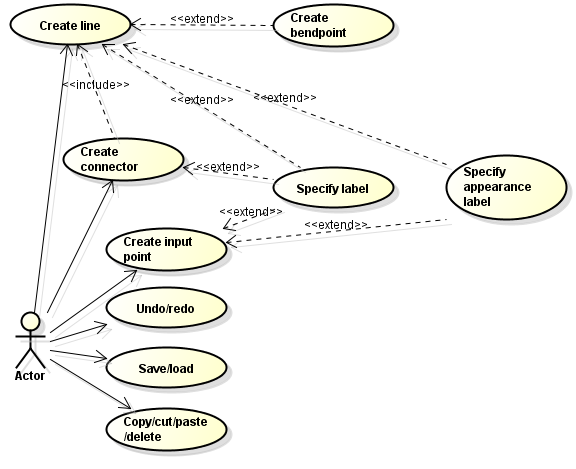
\includegraphics[width=0.5\textwidth]{image/uc-geometry.png}
  \caption{Use cases for the Geometry Editor }
  \label{fig:use-cases-geometry-editor}
\end{center}
\end{figure}